%
%intro
The stack implementation tests were mainly focused on the interactions established between the packages at play and the surrounding systems both lower-tiered and high-tiered.
%
\subsubsection{IO: Input/Output Package}
%
The IO package testing (figure \ref{fig:io-test}) consisted in the creation of a GPIO object with which one could simulate motor PWM outputs that would generate a file, through which one would simulate the IR sensor readings or motor pulse readings. The first GPIO test relied on a configuration of an object in OUTPUT\_PWM mode. With the latter test, it was possible to write three 32 bit integers to a binary file and observe the results with notepad++.
The second test hinged on reading from the forementioned binary file, expecting to retrieve the corresponding values. Should the latter be as expected the test could be considered a success.
%
\begin{figure}[!ht]
\centering
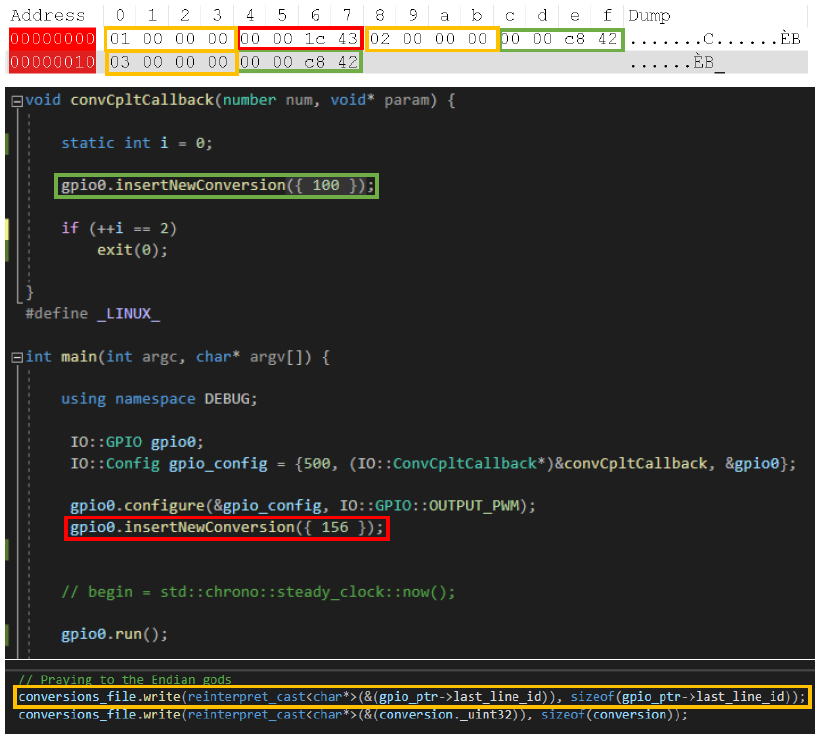
\includegraphics[width=0.8\textwidth]{img/IO-test.png}
\caption{\label{fig:io-test}IO package OUTPUT\_PMW mode tests}
\end{figure}
%
\subsubsection{COM: Communications Package}
%
The COM package testing involved effectuating some experiments between the \gls{nvs} and the smartphone (using Bluetooth) and the former and the \gls{rvvs} (using RS232). These experiments will be performed in section \ref{sec:nvs-tests}.
%
\subsubsection{OS: Scheduler Package}
%
The OS package testing was based on the creation of two types of Threads:
\begin{itemize}
	\item \textbf{Producer Thread (P)}
	\item \textbf{Consumer Thread (C)}
\end{itemize}
%
The OS package testing was based on the creation of two types of Threads. These tests were made to simulate the way how the operating system handles multi-thread contexts. The Producer Thread type publishes values in a list while the Consumer Thread type removes values from the latter. The introduction of an initial delay in the Producer Thread function allows the OS to assign the CPU more evenly.
The test is represented in figure \ref{fig:os-test}.
%
\begin{figure}[!ht]
\centering
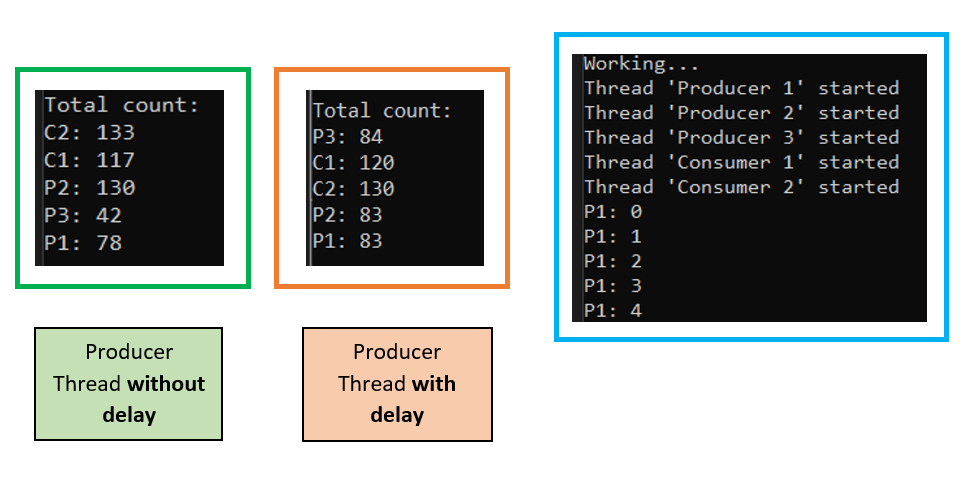
\includegraphics[width=0.8\textwidth]{img/OS-threads.png}
\caption{\label{fig:os-test}OS package tests}
\end{figure}
%
\subsubsection{MEM: Memory Structures Package}
%
The MEM Package testing consisted of creating two projects, one that used linked lists and another that used a circular buffer. In the former, one simply pushed numerical characters and verified that the appropriate memory spaces were filled. Afterwards, those characters were popped and the result was as expected, the memory spaces were removed from the list. This test is depicted in figure \ref{fig:fig:mem-test}.
%
\begin{figure}[!ht]
\centering
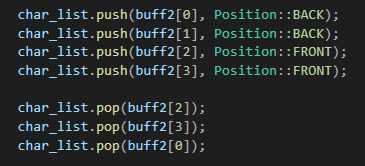
\includegraphics[width=0.6\textwidth]{img/MEM-linked-list.png}
\caption{\label{fig:mem-test}MEM package linked list tests excerpt}
\end{figure}
%
%
\subsubsection{CLK: Timing Package}
%
The CLK package testing (figure \ref{fig:clk-test}) included the creation of a Timer object, associating it to a callback and proceed to verify if the callback was called at the specified time preemptively defined in the Config object configuration.
%
\begin{figure}[!ht]
\centering
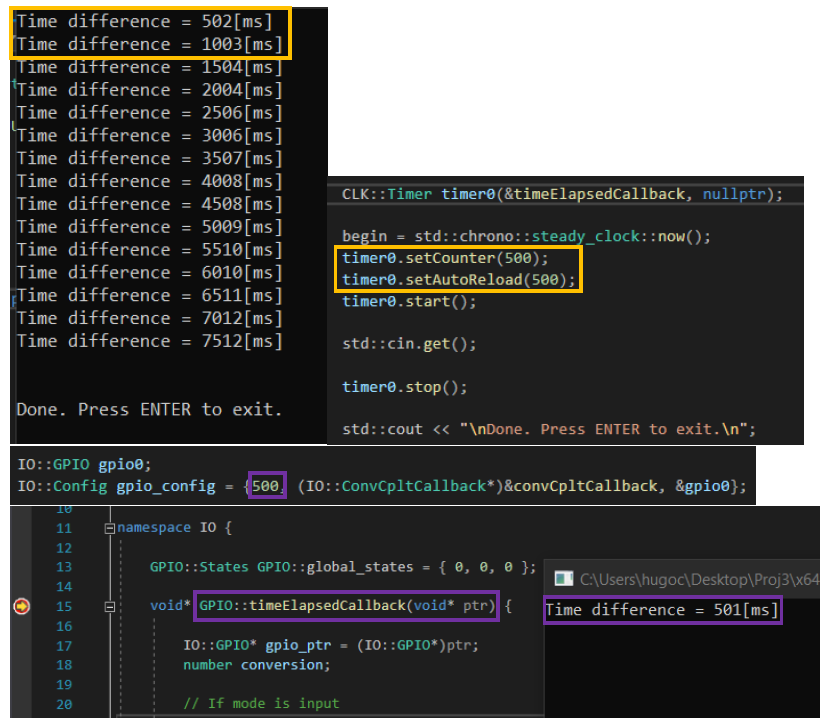
\includegraphics[width=0.8\textwidth]{img/CLK-test.png}
\caption{\label{fig:clk-test}CLK package tests}
\end{figure}
%